%
% teil1.tex -- Beispiel-File für das Paper
%
% (c) 2020 Prof Dr Andreas Müller, Hochschule Rapperswil
%
\section{Taylor-Approximation
\label{transfer:section:teil1}}
\subsection{Idee}
Die Taylorreihe kann eine glatte Funktion in einer Umgebung durch Polynome beliebig genau annähern. Beschränkt man sich auf einen bestimmten Grad dieser Polynome, spricht man von einer Taylor-Approximation. Diese entwickelt sich immer um einen Punkt und kann über die Ableitungen berechnet werden.

\subsection{Definition der Taylorreihe}
Sei $I \subset \mathbb{R}$ ein offenes Intervall, $f: I \rightarrow \mathbb{R}$ eine glatte Funktion und $a$ ein Element von $I$. Dann ist die unendliche Reihe
\begin{equation}
	T_{f(x ; a)}=\sum_{n=0}^{\infty} \frac{f^{(n)}(a)}{n !}(x-a)^{n}=f(a)+f^{\prime}(a)(x-a)+\frac{f^{\prime \prime}(a)}{2}(x-a)^{2}+\frac{f^{\prime \prime \prime}(a)}{6}(x-a)^{3}+\ldots
\end{equation}
die Taylorreihe von $f$ in Punkt $a$.

\subsection{Beispiel}
In diesem Beispiel wird die Taylor-Approximation mit dem Grad 2 des Tangens hyperbolicus um den Punkt Null berechnet.
$$
	\tanh(x) \approx T_{2} \tanh(x ; a)=\tanh(a)+\tanh^{\prime}(a) \cdot(x-a)+\frac{\tanh^{\prime \prime}(a) \cdot(x-a)^{2}}{2}
$$
mit $a = 0$ folgt
$$
	T_{2} \tanh(x ; 0)=\tanh(0)+\tanh^{\prime}(0) \cdot(x)+\frac{\tanh^{\prime \prime}(0) \cdot(x)^{2}}{2} = 0 + x + 0 = x.
$$
\begin{figure}
\centering
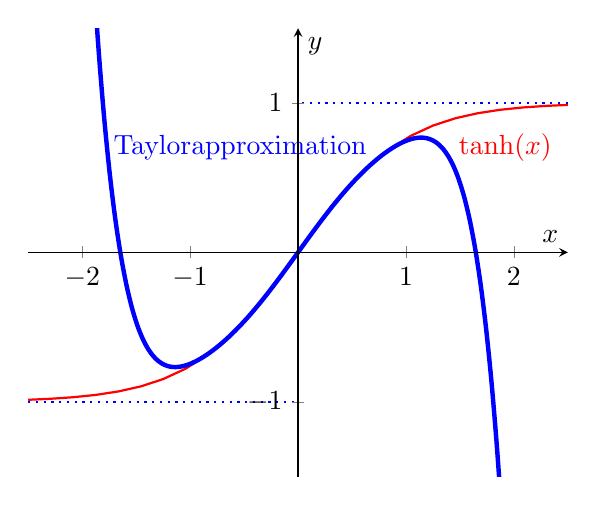
\begin{tikzpicture}
	\begin{axis}[
		xmin=-2.5, xmax=2.5,
		ymin=-1.5, ymax=1.5,
		axis lines=center,
		axis on top=true,
		domain=-2.5:2.5,
		ylabel=$y$,
		xlabel=$x$,
		]
		
		\addplot [mark=none,draw=red,thick] {tanh(\x)};
		\node [right, red] at (axis cs: 1.4,0.7) {$\tanh(x)$};
		\addplot [mark=none,draw=blue,ultra thick, samples=100, smooth] expression{x-(x^3)/3+ (2*x^5)/15-(17 * x^7)/315};
		\node [right, blue] at (axis cs: -1.8,0.7) {\text{Taylorapproximation}};
		
		%% Add the asymptotes
		\draw [blue, dotted, thick] (axis cs:-2.5,-1)-- (axis cs:0,-1);
		\draw [blue, dotted, thick] (axis cs:+2.5,+1)-- (axis cs:0,+1);
	\end{axis}
\end{tikzpicture}
\caption{Taylor-Approximation von Grad 7
\label{motivation:figure:Taylor}}
\end{figure}

\subsection{Vor- und Nachteile}
Im Vergleich mit dem klassischen Algorithmus ist die Berechnung der Taylorapproximation weniger aufwändig, dafür ist, wie in Abbildung \ref{motivation:figure:Taylor} ersichtlich, der Approximationsfehler sehr gross. Dies liegt unter anderem an der Unbeschränktheit, die solche Polynome besitzen. Für die Verwendung in neuronalen Netzwerken ist die Taylorapproximation deshalb nicht im Gebrauch.
